\documentclass{article}
\usepackage{graphicx}
\usepackage{geometry}
\usepackage{subcaption}
\usepackage{amsmath, amssymb}
\geometry{tmargin=3cm, lmargin=3cm, rmargin=2cm, bmargin=2cm}

\begin{document}
\section{Animals dataset}

Figure~\ref{fig:performance} shows how the results of estimating the graph Laplacian of the \textsf{animals} dataset
for different values of $K$. The \textsf{animals} dataset consists of binary values which are the answers to questions
such as "is warm-blooded?", "has lungs?", etc. There are in total 102 such questions (features) and 33 animals (nodes).

\begin{figure}[!htb]
    \centering
    \begin{subfigure}[b]{0.35\textwidth}
        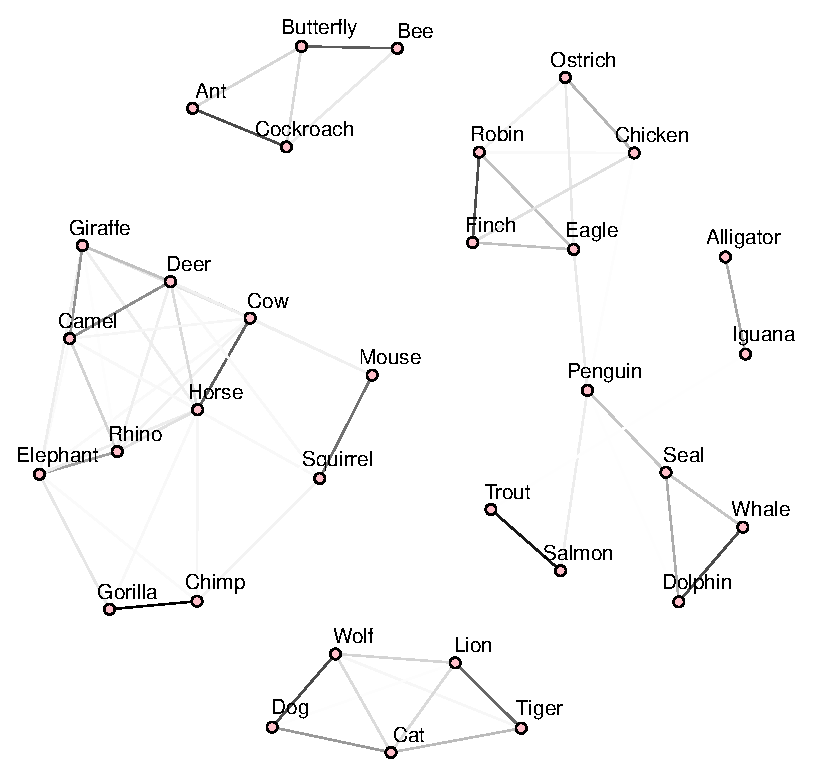
\includegraphics[width=\textwidth]{animals_graph_k1.eps}
        \caption{$K = 1$}
    \end{subfigure}
    ~
    \begin{subfigure}[b]{0.35\textwidth}
        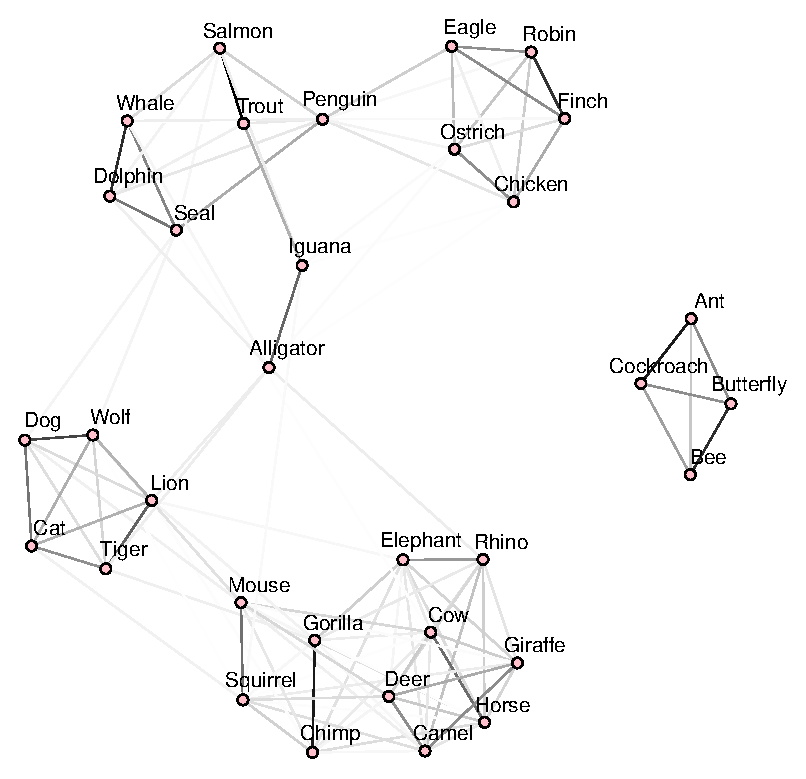
\includegraphics[width=\textwidth]{animals_graph_k2.eps}
        \caption{$K = 2$}
    \end{subfigure}
    ~
    \begin{subfigure}[b]{0.35\textwidth}
        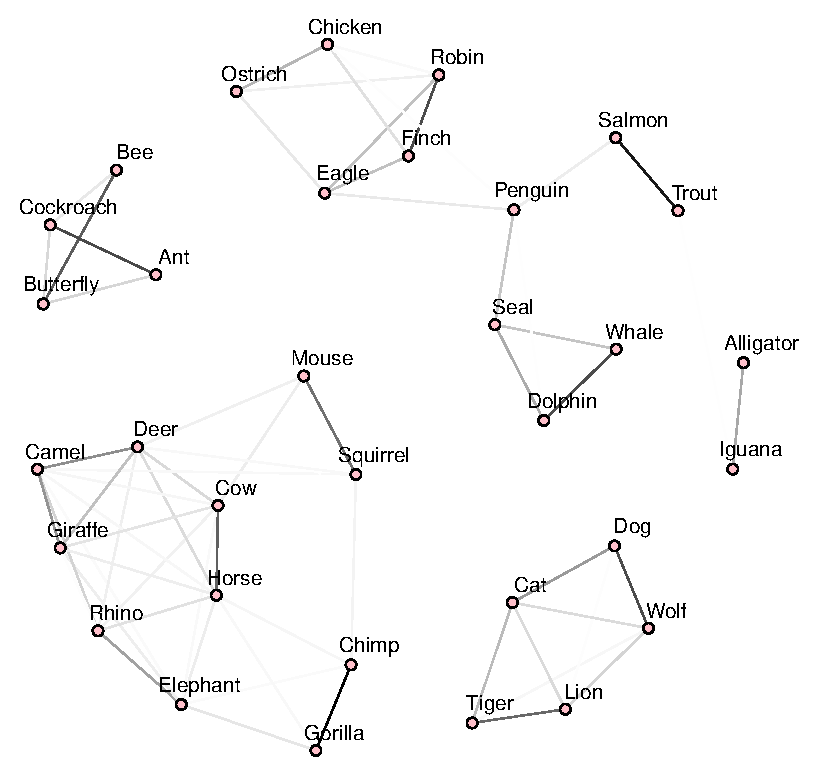
\includegraphics[width=\textwidth]{animals_graph_k4.eps}
        \caption{$K = 4$}
    \end{subfigure}
    ~
    \begin{subfigure}[b]{0.35\textwidth}
        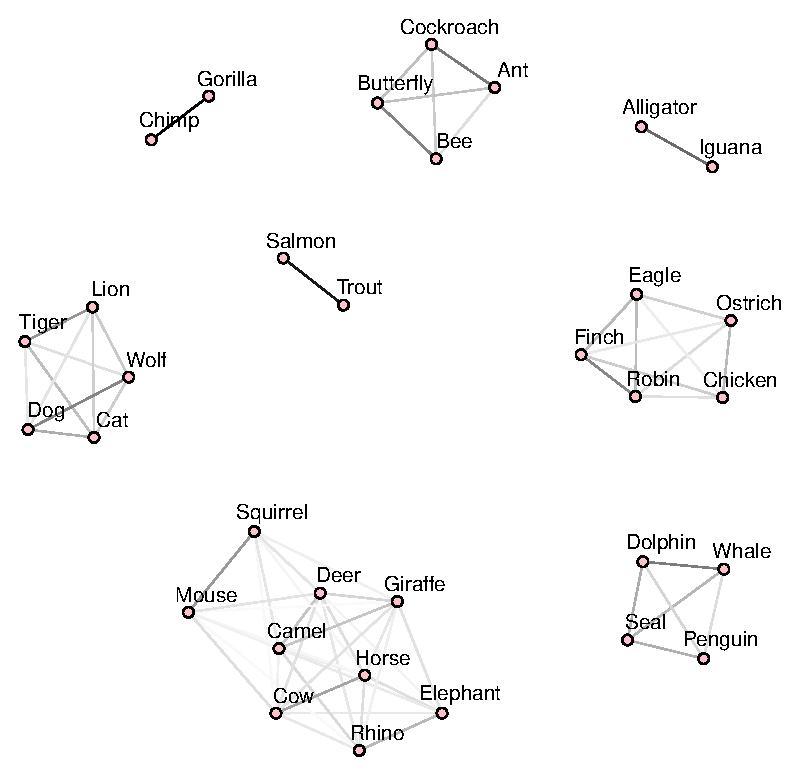
\includegraphics[width=\textwidth]{animals_graph_k8.eps}
        \caption{$K = 8$}
    \end{subfigure}
    ~
    \begin{subfigure}[b]{0.35\textwidth}
        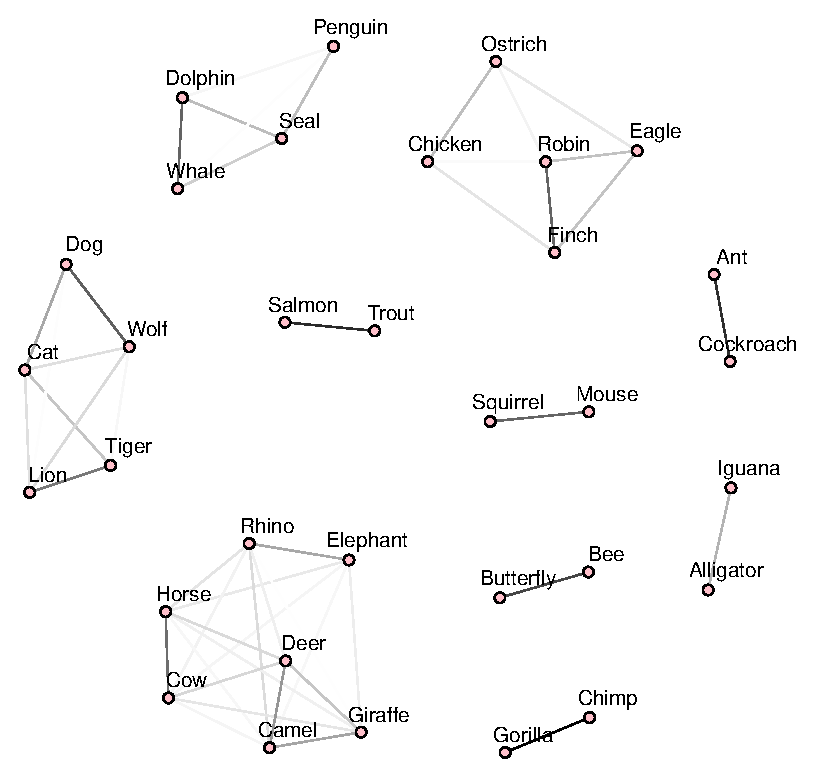
\includegraphics[width=\textwidth]{animals_graph_k10.eps}
        \caption{$K = 10$}
    \end{subfigure}
    \caption{Graph learning in the animals dataset for different values of $K$.}
    \label{fig:performance}
\end{figure}

\end{document}
